\documentclass{minimal}

\usepackage{pgfplots}
\pgfplotsset{compat=newest}
\usepgfplotslibrary{fillbetween}
\usepackage[eulergreek]{sansmath}


\pgfplotsset{
  tick label style = {font=\sansmath\sffamily},
  every axis label = {font=\sansmath\sffamily},
  legend style = {font=\sansmath\sffamily},
  label style = {font=\sansmath\sffamily}
}

\tikzset{every picture/.style={/utils/exec={\sansmath\sffamily}}}

\definecolor{takeoff}{RGB}{49, 130, 189}
\definecolor{landing}{RGB}{106,168,79}
\definecolor{limit}{RGB}{212,0,35}

\begin{document}

\pgfkeys{/pgf/number format/.cd,1000 sep={\,}}

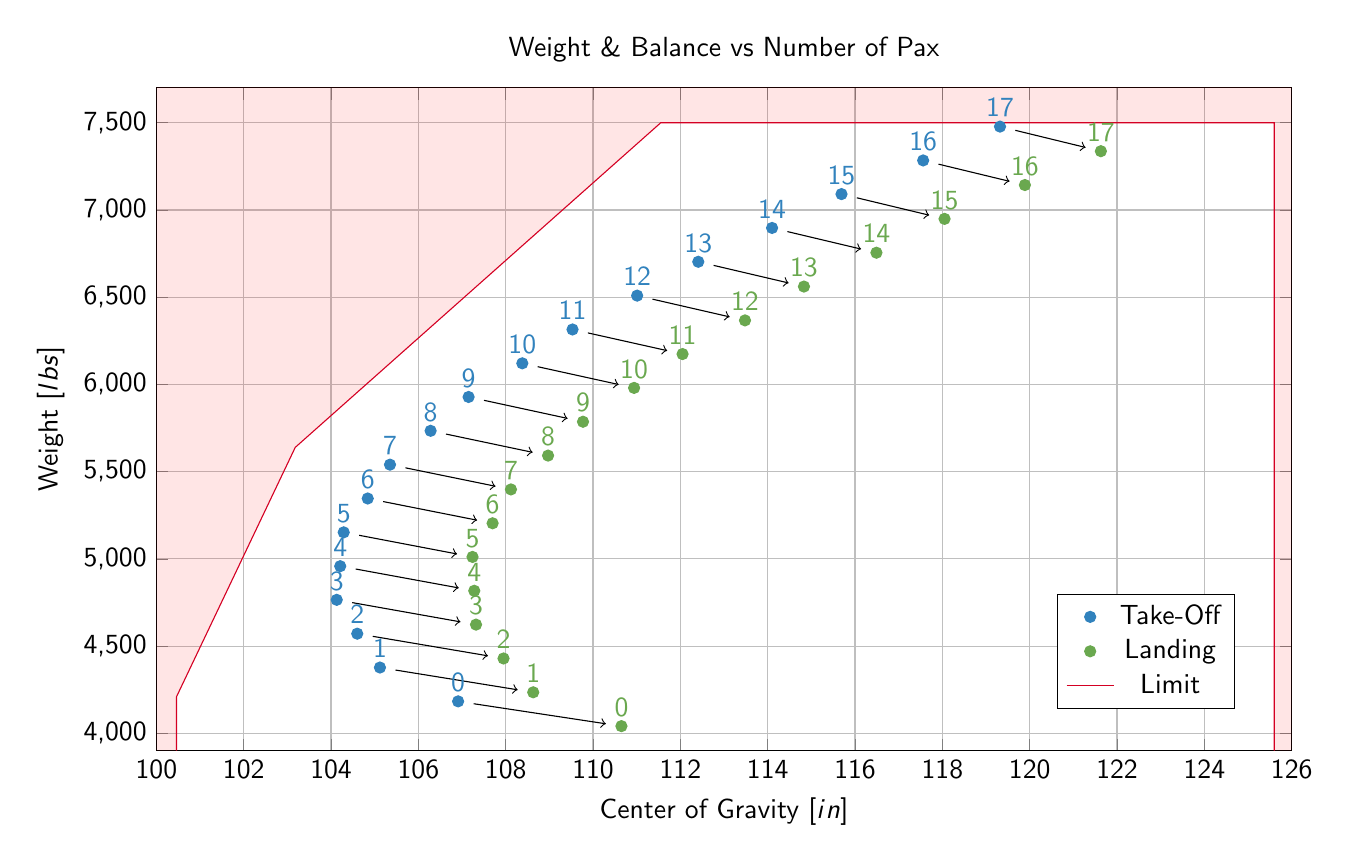
\begin{tikzpicture}
  \begin{axis}[
      title={Weight \& Balance vs Number of Pax},
      height=10cm,
      width=16cm,
      grid=major,
      nodes near coords,
      xlabel={Center of Gravity $[in]$},
      ylabel={Weight $[lbs]$},
      xmin=100,xmax=126,
      ymin=3900,ymax=7700,
      legend style={at={(0.95,0.15)},anchor=east}
    ]

    \addplot+[only marks,
      mark=*,
      mark options={scale=1, fill=takeoff},
      color=takeoff,
      point meta=explicit symbolic
    ] coordinates {
      (106.91,4183) [0]
      (105.12,4377) [1]
      (104.60,4571) [2]
      (104.13,4765) [3]
      (104.21,4958) [4]
      (104.29,5152) [5]
      (104.84,5346) [6]
      (105.35,5540) [7]
      (106.28,5734) [8]
      (107.15,5928) [9]
      (108.38,6121) [10]
      (109.53,6315) [11]
      (111.01,6509) [12]
      (112.41,6703) [13]
      (114.10,6897) [14]
      (115.69,7091) [15]
      (117.56,7284) [16]
      (119.32,7478) [17]
    };
    \addlegendentry{Take-Off}

    \addplot+[only marks,
      mark=*,
      mark options={scale=1, fill=landing},
      color=landing,
      point meta=explicit symbolic
    ] coordinates {
      (110.65,4041) [0]
      (108.63,4235) [1]
      (107.95,4429) [2]
      (107.32,4623) [3]
      (107.28,4817) [4]
      (107.24,5011) [5]
      (107.70,5204) [6]
      (108.12,5398) [7]
      (108.97,5592) [8]
      (109.77,5786) [9]
      (110.94,5980) [10]
      (112.05,6174) [11]
      (113.48,6367) [12]
      (114.83,6561) [13]
      (116.49,6755) [14]
      (118.05,6949) [15]
      (119.89,7143) [16]
      (121.63,7337) [17]
    };
    \addlegendentry{Landing}

    \addplot+[mark=none,
      color=limit,
      point meta=explicit symbolic
    ] coordinates {
      (100.46, 3900) []
      (100.46, 4209) []
      (103.18, 5639) []
      (111.55, 7500) []
      (125.60, 7500) []
      (125.60, 3900) []
    };
    \addlegendentry{Limit}

    \addplot+[mark=none,
      draw=none,
      point meta=explicit symbolic,
      name path=limit-top] coordinates {
      (100.00, 3900) []
      (100.46, 3900) []
      (100.46, 4209) []
      (103.18, 5639) []
      (111.55, 7500) []
      (125.60, 7500) []
      (125.60, 3900) []
      (130.00, 3900) []
    };

    \path[name path=top] (100,8000) -- (130,8000);
    \addplot[red, fill opacity=0.1] fill between[of=top and limit-top];

    \draw [->,shorten >=2mm, shorten <=2mm] (106.91,4183) -- (110.65,4041);
    \draw [->,shorten >=2mm, shorten <=2mm] (105.12,4377) -- (108.63,4235);
    \draw [->,shorten >=2mm, shorten <=2mm] (104.60,4571) -- (107.95,4429);
    \draw [->,shorten >=2mm, shorten <=2mm] (104.13,4765) -- (107.32,4623);
    \draw [->,shorten >=2mm, shorten <=2mm] (104.21,4958) -- (107.28,4817);
    \draw [->,shorten >=2mm, shorten <=2mm] (104.29,5152) -- (107.24,5011);
    \draw [->,shorten >=2mm, shorten <=2mm] (104.84,5346) -- (107.70,5204);
    \draw [->,shorten >=2mm, shorten <=2mm] (105.35,5540) -- (108.12,5398);
    \draw [->,shorten >=2mm, shorten <=2mm] (106.28,5734) -- (108.97,5592);
    \draw [->,shorten >=2mm, shorten <=2mm] (107.15,5928) -- (109.77,5786);
    \draw [->,shorten >=2mm, shorten <=2mm] (108.38,6121) -- (110.94,5980);
    \draw [->,shorten >=2mm, shorten <=2mm] (109.53,6315) -- (112.05,6174);
    \draw [->,shorten >=2mm, shorten <=2mm] (111.01,6509) -- (113.48,6367);
    \draw [->,shorten >=2mm, shorten <=2mm] (112.41,6703) -- (114.83,6561);
    \draw [->,shorten >=2mm, shorten <=2mm] (114.10,6897) -- (116.49,6755);
    \draw [->,shorten >=2mm, shorten <=2mm] (115.69,7091) -- (118.05,6949);
    \draw [->,shorten >=2mm, shorten <=2mm] (117.56,7284) -- (119.89,7143);
    \draw [->,shorten >=2mm, shorten <=2mm] (119.32,7478) -- (121.63,7337);

  \end{axis}
\end{tikzpicture}


\end{document}
